\documentclass[conf]{new-aiaa}
%\documentclass[journal]{new-aiaa} for journal papers
\usepackage[utf8]{inputenc}

\usepackage{graphicx}
\usepackage{amsmath}
\usepackage{commath}
\usepackage[version=4]{mhchem}
\usepackage{siunitx}
\usepackage{longtable,tabularx}
\usepackage{float}
\usepackage{listings}
\usepackage{pdfpages}
\usepackage{color} %red, green, blue, yellow, cyan, magenta, black, white
\definecolor{mygreen}{RGB}{28,172,0} % color values Red, Green, Blue
\definecolor{mylilas}{RGB}{170,55,241}
\setlength\LTleft{0pt} 

\lstset{language=Matlab,%
	basicstyle=\footnotesize,
	breaklines=true,%
	morekeywords={matlab2tikz},
	keywordstyle=\color{blue},%
	morekeywords=[2]{1}, keywordstyle=[2]{\color{black}},
	identifierstyle=\color{black},%
	stringstyle=\color{mylilas},
	commentstyle=\color{mygreen},%
	showstringspaces=false,%without this there will be a symbol in the places where there is a space
	numbers=left,%
	numberstyle={\tiny \color{black}},% size of the numbers
	numbersep=9pt, % this defines how far the numbers are from the text
	emph=[1]{for,end,break},emphstyle=[1]\color{red}, %some words to emphasise
	%emph=[2]{word1,word2}, emphstyle=[2]{style},    
}

% ================================================================ % 
\title{ASE387P.2 Mission Analysis and Design \\ Homework 3}

\author{Junette Hsin}
\affil{Masters Student, Aerospace Engineering and Engineering Mechanics, University of Texas, Austin, TX 78712}

\begin{document}

\maketitle

% \begin{abstract}

	% Theory and algorithms 

% \end{abstract}

% \newpage 
% ================================================================ % 
\section*{Problem 1}

\textbf{All analyses for this section are for a desired 60 degree transfer angle in the clockwise direction from the initial / departure position.} \\ 

The desired transfer angle of 60 degrees was defined to be the angle between the initial / departure longitude and the final / arrival longitude. 

\begin{equation}
    \Delta L_{des} = L_{M_f} - L_{E_i}
    \label{eq:DL}
\end{equation}

For an outbound transfer, the initial longitude would be Earth and the final longitude would be Mars. For inbound transfer, the initial longitude would be Mars and the final longitude would be Earth. Equation \ref{eq:DL} could also be rewritten as: 

\begin{equation}
    L_{M_f} = \Delta L_{des} + L_{E_i}
    \label{eq:Lf1}
\end{equation}

The final longitude can also be found from the motion of the planets: 

\begin{equation}
    L_{M_f} = L_{M_i} + \Delta t \dot{L_{M}}
    \label{eq:Lf2}
\end{equation}

Combing Equations \ref{eq:Lf1} and \ref{eq:Lf2} result in: 

\begin{equation}
    \Delta t = \frac{\Delta L_{des} + L_{E_i} - L_{M_i}}{ \dot{L_M} }
\end{equation}

The document \textbf{aprx\_pos\_planets.pdf} was used to compute the orbital elements and Cartesian states of Earth and Mars. Once $\Delta t$ and an initial time are known, the positions of the planets are known. The Lambert solver from HW 2 was used to find the time of flight for the minimum energy transfer. 

The above algorithm was iterated until the TOF for the minimum energy transfer aligned with the time for a 60 degree transfer angle between departure and arrival positions to develop. For example, for an outbound trajectory from Earth to Mars, the 60 degree transfer angle is computed between the initial Earth position and the final Mars position. However, Mars still has an initial position, and will take some amount of time which we will call $\Delta t_M$ to reach its final position. The algorithm was iterated until the TOF for the minimum energy transfer aligned with $\Delta t_M$.  


% ------------------------- % 
\subsection*{A}

To calculate the synodic period, first, the period of Mars was calculated in years: 

\begin{equation}
    T_{Mars} = \frac{1}{\dot{L}_{Mars}} \times \frac{100 \; years}{1 \; century} \times \frac{360 ^\circ}{1 \; rev}
\end{equation}

The synodic period was then calculated with the following equation: 

\begin{equation}
    SP_{Mars} = \frac{T_{Mars}}{|| T_{Mars} - 1 ||}
\end{equation}

The synodic period came out to be 2.13526965089401. 

% ------------------------- % 
\subsection*{B}

The launch date (T0), arrival date (T1), and the time of flight for the 1st launch window are displayed in the figure below. 

\begin{figure}[H]
    \centering 
    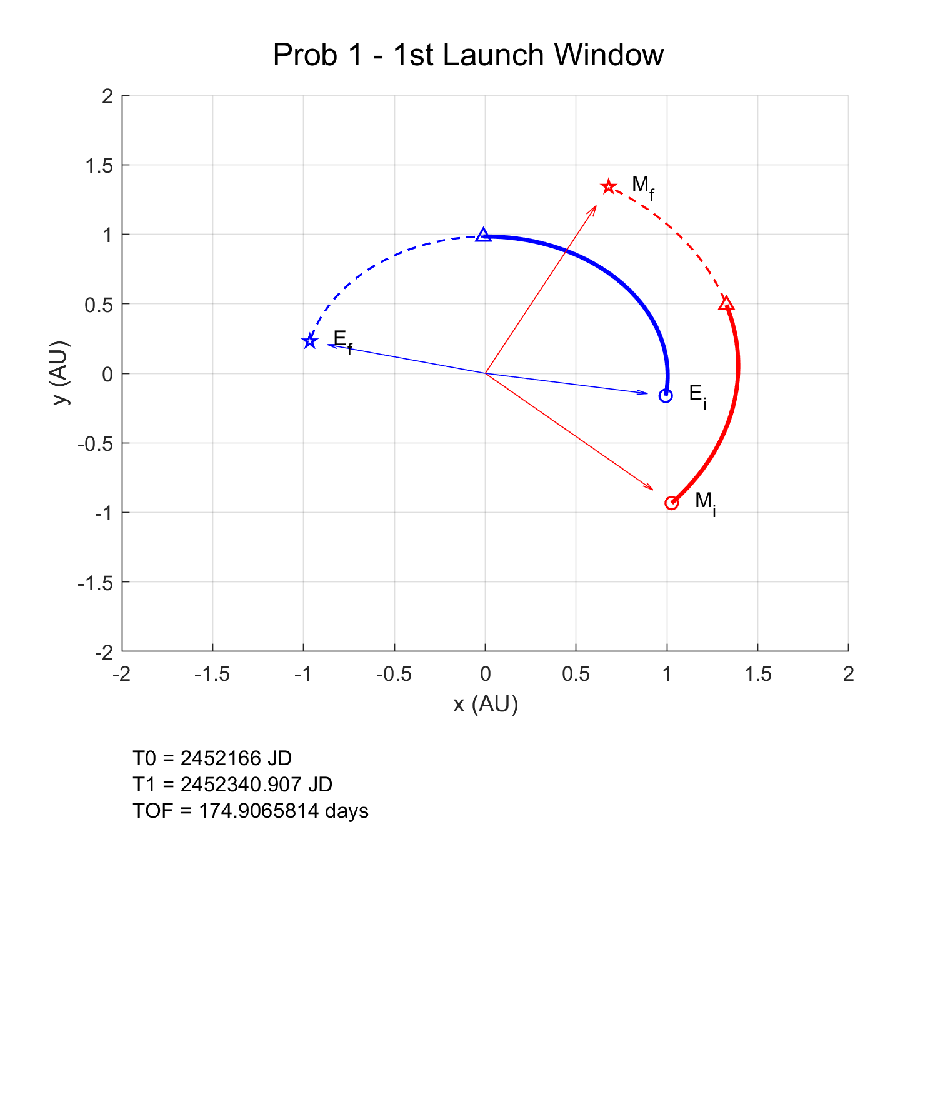
\includegraphics[width=0.7\textwidth]{Prob 1 - 1st Launch Window.pdf}
    \caption{1st Earth to Mars 60 degrees transfer}
\end{figure}

The launch date (T0), arrival date (T1), and the time of flight for the 2nd launch window are displayed in the figure below. 

\begin{figure}[H]
    \centering 
    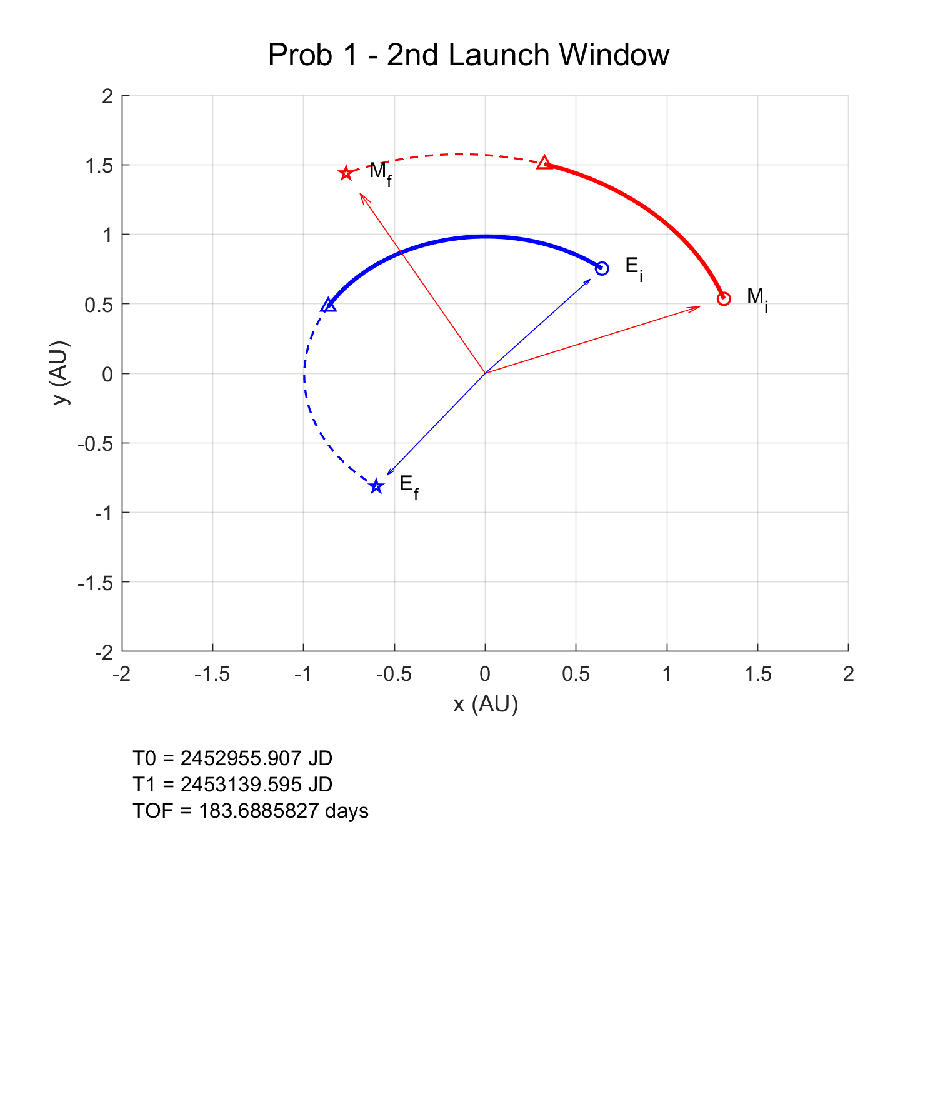
\includegraphics[width=0.7\textwidth]{Prob 1 - 2nd Launch Window.pdf}
    \caption{2nd Earth to Mars 60 degrees transfer}
\end{figure}

% ------------------------- % 
\subsection*{C}

The launch date (T0), arrival date (T1), and the time of flight for the 2nd launch window are displayed in the figure below. 

\begin{figure}[H]
    \centering 
    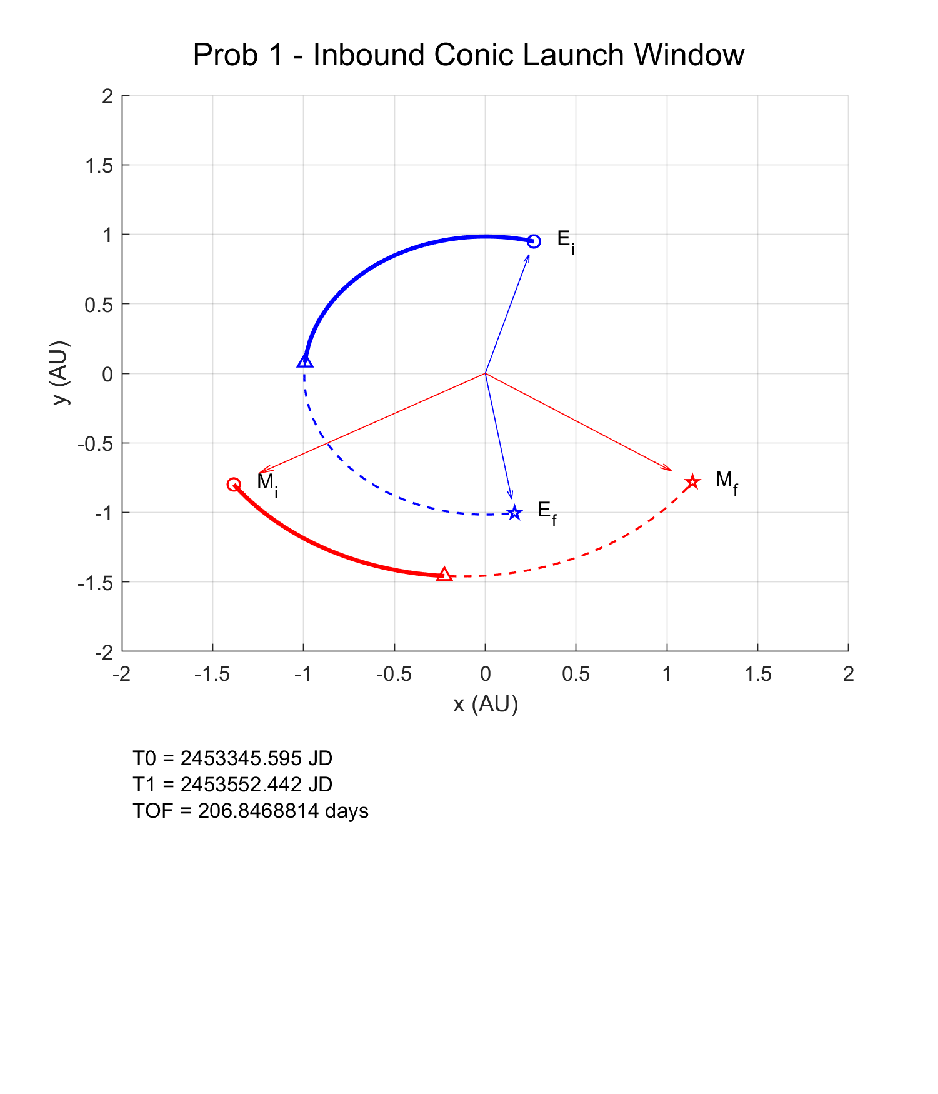
\includegraphics[width=0.7\textwidth]{Prob 1 - Inbound Conic Launch Window.pdf}
    \caption{Inbound Mars to Earth 60 degrees transfer}
\end{figure}

% \newpage 
% ================================================================ % 
\section*{Problem 2}

\subsection*{A}
In the previous section, the angle between Earth and Mars was computed using the approximate longitude from \textbf{aprx\_pos\_planets.pdf}. For Problem 2, the 1.85 $^\circ$ inclination of Mars' orbit was factored into the angle calculation. \\ 

The angle between the Earth and Mars position vectors was calculated using dot product. Then, the desired angle between initial Mars and final Mars position was computed. The mean change in longitude rate from \textbf{aprx\_pos\_planets.pdf} was still used to determine the time for the desired arrival planet to go from its initial position to desired final position. \\ 

The launch date (T0), arrival date (T1), and the time of flight for the 2nd launch window are displayed in the figure below. \textbf{The z axis is zoomed in to show the exaggerated inclination of Mars' orbit.}

\begin{figure}[H]
    \centering 
    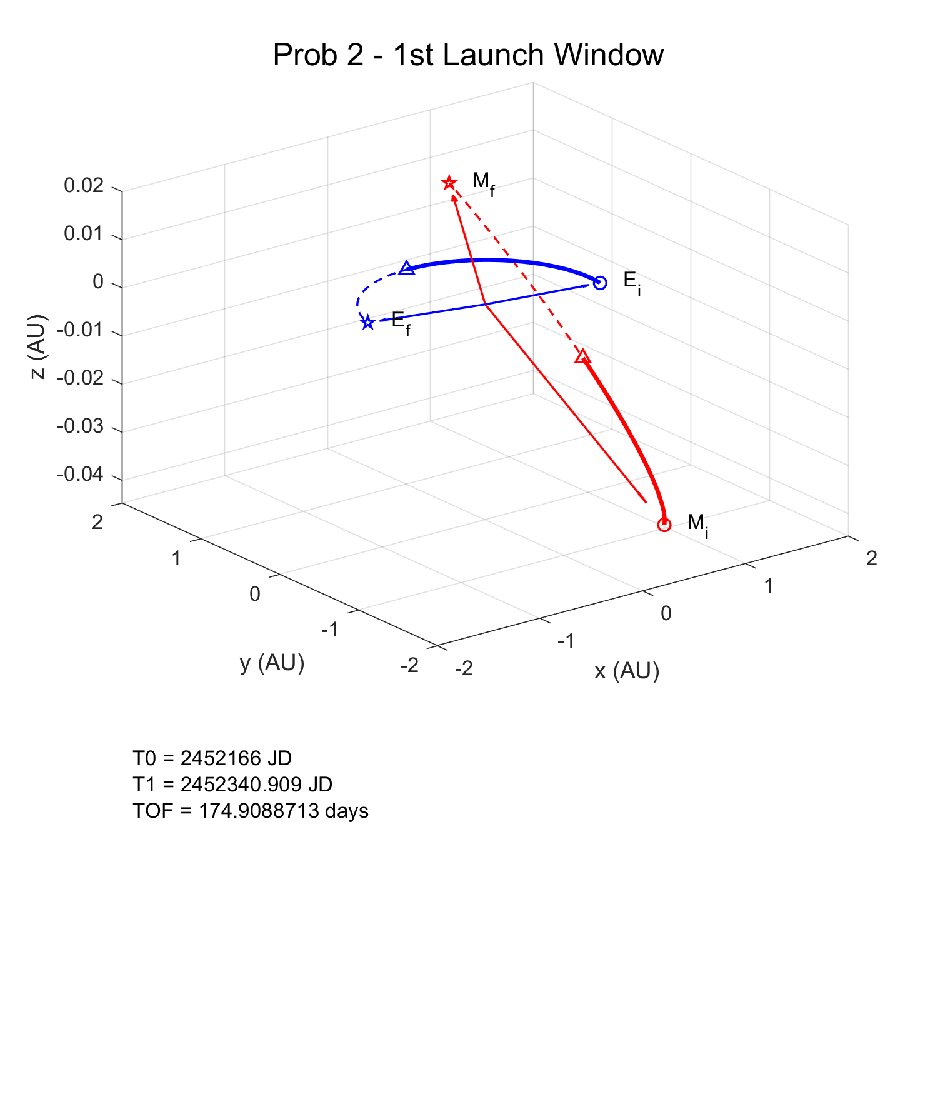
\includegraphics[width=0.7\textwidth]{Prob 2 - 1st Launch Window.pdf}
    \caption{1st Earth to Mars 60 degrees transfer with Mars inclination}
\end{figure}

\begin{figure}[H]
    \centering 
    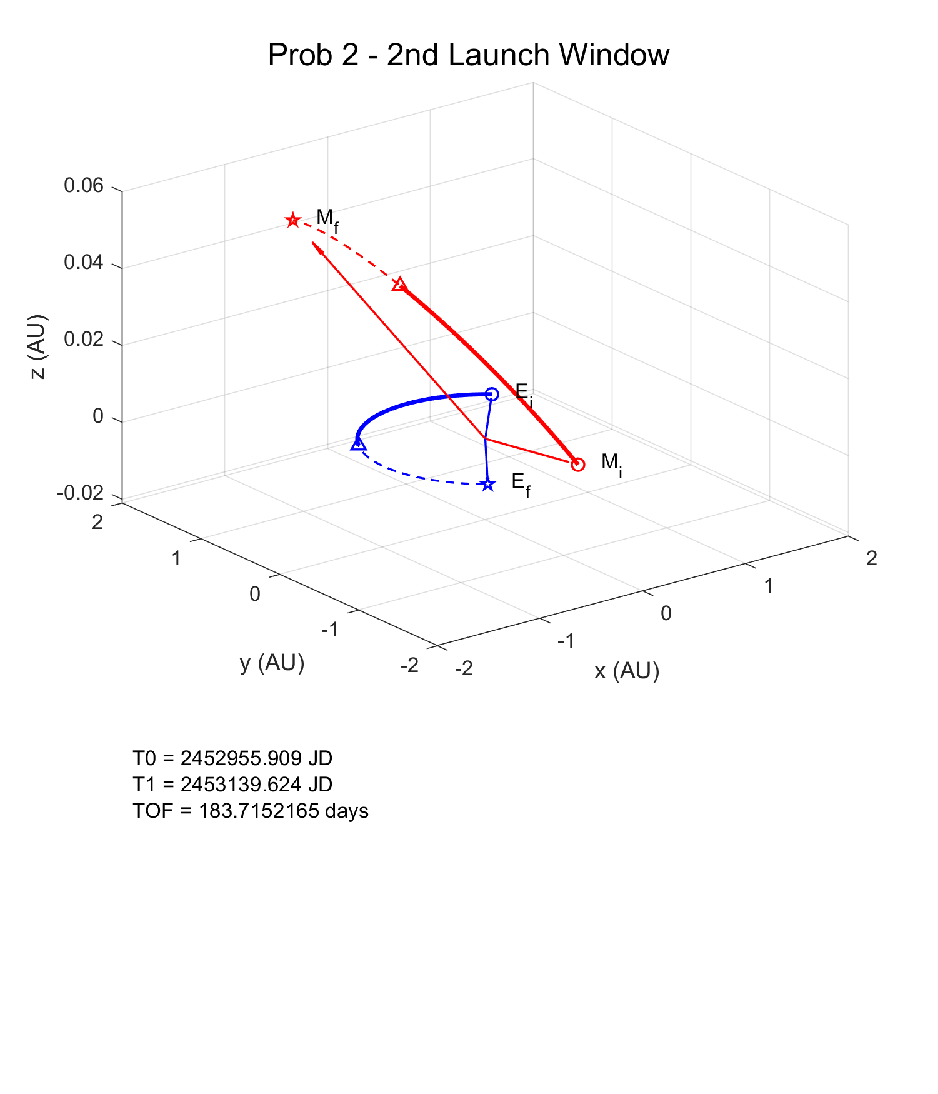
\includegraphics[width=0.7\textwidth]{Prob 2 - 2nd Launch Window.pdf}
    \caption{2nd Earth to Mars 60 degrees transfer with Mars inclination}
\end{figure}

\begin{figure}[H]
    \centering 
    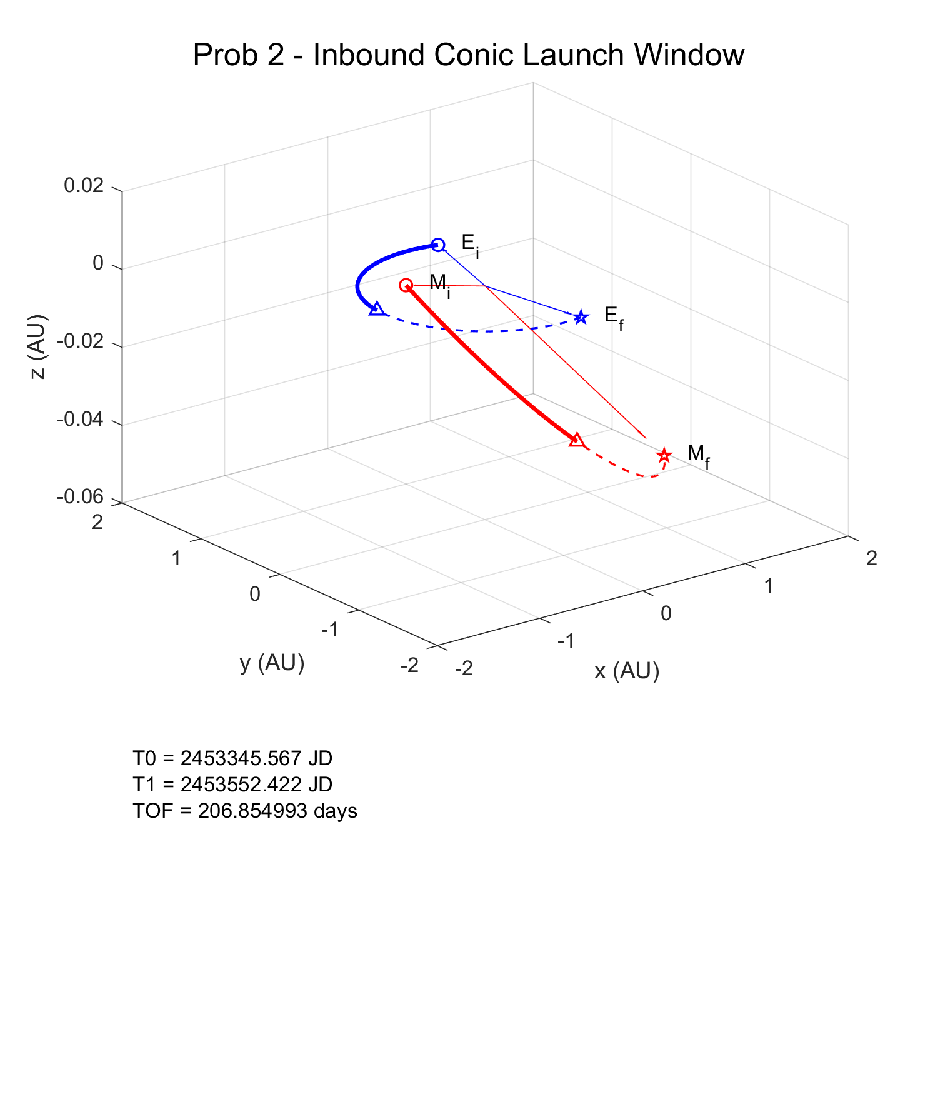
\includegraphics[width=0.7\textwidth]{Prob 2 - Inbound Conic Launch Window.pdf}
    \caption{Inbound Mars to Earth 60 degrees transfer with Mars inclination}
\end{figure}

% ------------------------- % 
\subsection*{B}

% ================================================================ % 
% Problem 3 

\newpage
% ================================================================ % 
\section*{Appendix} 

\subsection*{MATLAB code} 

\begin{lstlisting}

    
	
\end{lstlisting}





% ================================================================ % 

% \bibliography{sample}

\end{document}
